%\documentclass[12pt]{article}
%\usepackage[a4paper, margin=1in]{geometry} 
%\usepackage{graphicx} 
%\usepackage{hyperref}
%\usepackage{float}
%\usepackage{multicol}
%\usepackage{multirow}
%\usepackage[font=small, labelfont=bf]{caption}
%
%\begin{document} 

%
% Finite-state machine with n-grams
%
\subsection{Finite-state machine with n-grams}
Finite-state machine enables efficient database search by expanding the basic n-gram based search.

%
% Number of potential matching n-grams
%
\subsubsection*{Number of potential matching n-grams} 
The number of potential n-grams increases by the alphabet size and the word size.

\medskip 

\noindent
\textbf{DNA} \\
C = \{A, C, G, T\} \\
Word size 2  $\rightarrow$ $4^2$ = 16 \\
Word size 3  $\rightarrow$ $4^3$ = 64 \\
Word size 12  $\rightarrow$ $4^{12}$ = 16,777,216 \\

\noindent
\textbf{Protein} \\
C = \{A, R, N, D, C, Q, E, G, H, I, L, L, M, F, P, S, T, W, Y, V\} \\
Word size 2  $\rightarrow$ $20^2$ = 400 \\
Word size 3  $\rightarrow$ $20^3$ = 8000

%
% Number of potential matching n-grams
%
\subsubsection*{Finite-state machine} 
A finite-state machine can be used to scan database sequences instead of using a lookup table. Finite-state machines are usually faster than lookup tables.

\begin{figure}[H]
  \centering
      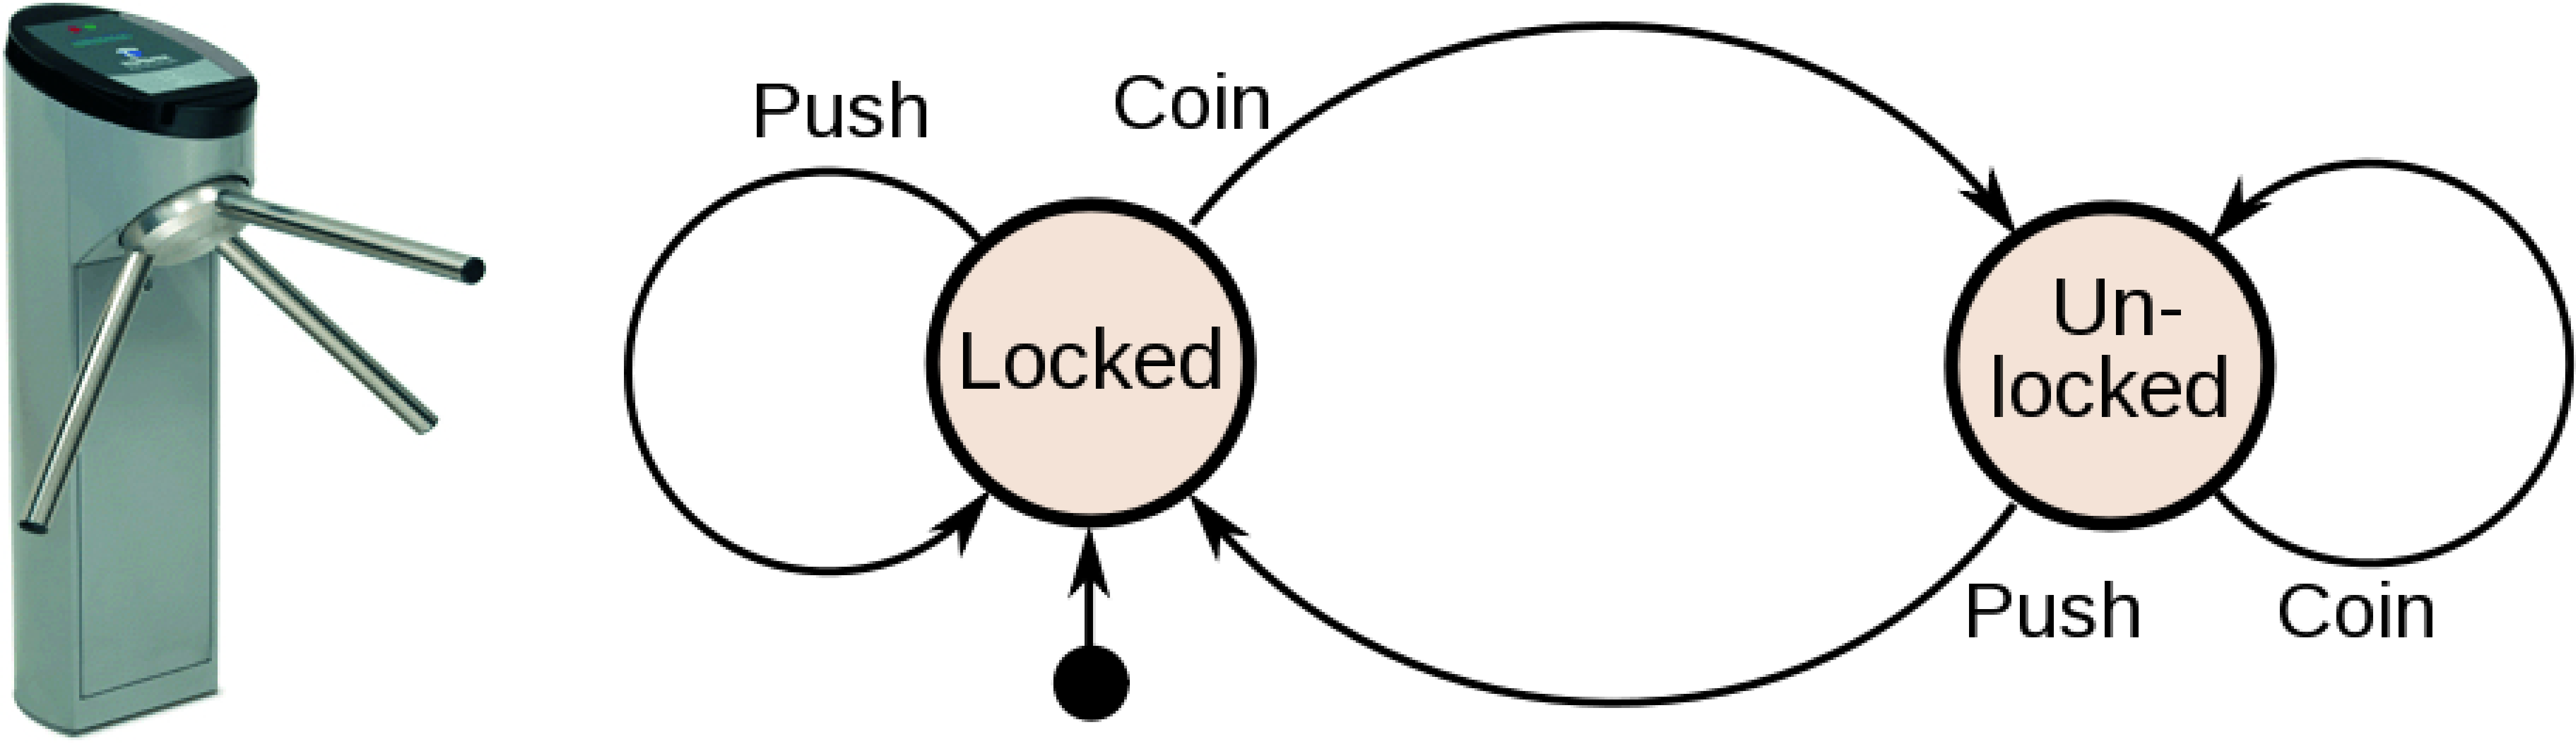
\includegraphics[width=0.6\textwidth]{fig05/fsm_turnstile.png}
  \caption{Finite-state machine for coin-operated turnstile  \newline (sources: \href{https://commons.wikimedia.org/w/index.php?curid=20269475}{Chetvorno} and \href{https://commons.wikimedia.org/w/index.php?curid=8930080}{Sebasgui} via Wikimedia Commons)}
\end{figure}

%
% Example of creating a FSM
%
\subsubsection*{Example of creating a finite-state machine} 

\begin{verbatim}
    q: ACGTAC, Word size: 2, T: 3
\end{verbatim} 

Lookup table
\begin{table}[H]
\small
\begin{tabular}{|l|l|l|}
\hline
\textbf{Matching n-gram} & \textbf{Indices of q} & \textbf{Scores of segment pairs} \\ \hline
AC                       & 1, 5                  & 4, 4                             \\ \hline
GC                       & 1, 3, 5               & 3, 3, 3                          \\ \hline
AT                       & 1, 3, 5               & 3, 3, 3                          \\ \hline
CG                       & 2                     & 4                                \\ \hline
TG                       & 2, 4                  & 3, 3                             \\ \hline
CA                       & 2, 4                  & 3, 3                             \\ \hline
GT                       & 3                     & 4                                \\ \hline
TA                       & 4                     & 4                                \\ \hline
\end{tabular}
\end{table}


\begin{figure}[H]
  \centering
      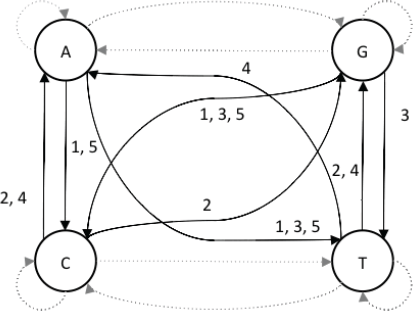
\includegraphics[width=0.4\textwidth]{fig05/fsm_example.png}
  \caption{Finite-state machine to output the indices of 2-grams}
\end{figure}

\begin{verbatim}
    d1: AAAGTG 
    
    2 hits
    GT – index: 3
    TG – index: (2, 4)
\end{verbatim}

%
% Exercise \thesection.2
%
\subsubsection*{Exercise \thesection.2}
Create a finite-state machine and use it to find a segment pair.


\begin{enumerate}
\item Create a finite-state machine for the lookup table for q: ACGTAC. Add both indices and scores to the edges.

\medskip 
Lookup table
\begin{table}[H]
\centering
\small
\begin{tabular}{|l|l|l|}
\hline
\textbf{Matching n-gram} & \textbf{Indices of q} & \textbf{Scores of segment pairs} \\ \hline
AC                       & 1, 5                  & 2, 2                             \\ \hline
CG                       & 2                     & 4                                \\ \hline
GT                       & 3                     & 2                                \\ \hline
TA                       & 4                     & 0                                \\ \hline
\end{tabular}
\end{table}

\item Use the finite-state machine and find a segment pair between q and d: AAAGTG.
\end{enumerate}

\bigskip 

%\end{document}
